\documentclass{if-beamer}
\usepackage[utf8]{inputenc}
\usepackage[T1]{fontenc}
% --------------------------------------------------- %
%                  Presentation info	              %
% --------------------------------------------------- %
\title[Pesquisa Operacional]{Ultralytics YOLO: Visão Computacional para Engenharia e Agricultura de Precisão}
\subtitle{Aplicações e Desempenho}
\author[Haron Calegari Fanticelli]{\large \negrito{Leonardo de Andrade Santos}}
\institute[UFPR]{
    \small \textit{Universidade Federal do Paraná} \\
    \textit{Curitiba}
}
\date{\today}
\logo{

\includegraphics[scale=.1, clip]{ufpr.png}
}
\subject{Presentation subject} % metadata
%trim={<left> <lower> <right> <upper>}
\graphicspath{{figuras/}}
% --------------------------------------------------- %
%                    Title + Schedule                 %
% --------------------------------------------------- %

\begin{document}
	
	\begin{frame}
		\titlepage
	\end{frame}
	
	\begin{frame}{Sumário}
		\tableofcontents
	\end{frame}
	
	% Section 1: Introdução
	\section{Introdução}
	
	\begin{frame}{Contexto da Visão Computacional}
		\begin{itemize}
			\item Visão computacional otimiza processos em engenharia e agricultura.
			\item Foco em agricultura de precisão: sustentabilidade e eficiência de recursos.
			\item Monitoramento de infraestrutura com análise visual avançada.
			\item Desafios: qualidade de imagens, sobreposição de plantas em VANTs.
		\end{itemize}
	\end{frame}
	
	\begin{frame}{Objetivo do Estudo}
		\begin{itemize}
			\item Apresentar a biblioteca Ultralytics YOLO como solução para:
			\begin{itemize}
				\item Detecção e segmentação de objetos em tempo real.
				\item Aplicações em agricultura (ex.: análise de plantações de soja).
				\item Monitoramento de infraestrutura (ex.: chaves seccionadoras).
			\end{itemize}
			\item Demonstrar desempenho e flexibilidade do YOLOv11.
		\end{itemize}
	\end{frame}
	
	% Section 2: Metodologia
	\section{Metodologia}
	
\begin{frame}{O Algoritmo YOLO}
	\begin{columns}[T]
		\begin{column}{0.5\textwidth}
			\begin{itemize}
				\item \textbf{You Only Look Once (YOLO)}: abordagem unificada para detecção de objetos.
				\item Reformula detecção como problema de regressão via CNN.
				\item Processo:
				\begin{enumerate}
					\item Divide imagem em grade $S \times S$.
					\item Cada célula prevê $B$ caixas delimitadoras e probabilidades de classe.
					\item Pontuação de confiança: $\mathrm{Pr}(\text{Objeto}) \times \text{IoU}_{\text{truth}}^{\text{pred}}$.
				\end{enumerate}
			\end{itemize}
		\end{column}
		\begin{column}{0.5\textwidth}
			\begin{figure}
				\centering
				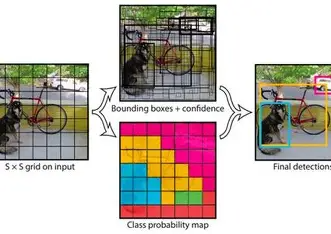
\includegraphics[width=\textwidth]{figuras/yolo.png}
				\caption{Exemplo de detecção de objetos com YOLO, mostrando caixas delimitadoras em uma imagem.}
				\label{fig:yolo_example}
			\end{figure}
		\end{column}
	\end{columns}
\end{frame}
	
	\begin{frame}{Funcionamento do YOLO}
		\begin{itemize}
			\item \textbf{Parâmetros por caixa}: $(x, y, w, h, \text{confiança})$.
			\item \textbf{Probabilidades de classe}: $\mathrm{Pr(Class_i | Object)}$.
			\item \textbf{Pontuação final}: 
			\[
			\mathrm{Pr(Class_i | Object)} \times \mathrm{Pr(Object)} \times \text{IoU}.
			\]
			\item Vantagens:
			\begin{itemize}
				\item Velocidade: 45–155 fps.
				\item Raciocínio global: analisa imagem completa.
				\item Generalização: robusto em novos domínios.
			\end{itemize}
		\end{itemize}
	\end{frame}
	
	\begin{frame}[fragile]{Ultralytics YOLO}
		\begin{itemize}
			\item Versão avançada do YOLO, com suporte a:
			\begin{itemize}
				\item Detecção, segmentação, classificação, estimativa de pose, rastreamento.
			\end{itemize}
			\item \textbf{Instalação}: 
			\[
			\texttt{pip install ultralytics}
			\]
			\item \textbf{Treinamento}: Suporta fine-tuning com datasets personalizados.
			\item \textbf{Exemplo de código}:
			\begin{verbatim}
				from ultralytics import YOLO
				model = YOLO("yolov11n.pt")
				model.train(data="dataset.yaml", epochs=10, imgsz=640)
			\end{verbatim}
		\end{itemize}
	\end{frame}
	
	% Section 3: Resultados
	\section{Resultados}
	
	\begin{frame}{Experimento: Identificação de Veículos}
		\begin{itemize}
			\item \textbf{Conjunto de dados}: Imagens urbanas com veículos.
			\item \textbf{Modelo}: YOLOv11 pré-treinado.
			\item \textbf{Métricas}:
			\begin{itemize}
				\item Alta precisão média (mAP) em boas condições de iluminação.
				\item Detecção robusta de caixas delimitadoras.
			\end{itemize}
			\item \textbf{Resultado visual}: Caixas delimitadoras com pontuações de confiança.
		\end{itemize}
	\end{frame}
	
	\begin{frame}{Desempenho do YOLOv11}
		\begin{table}
			\centering
			\begin{tabular}{l|c}
				\hline
				\textbf{Métrica} & \textbf{Valor} \\
				\hline
				Velocidade (fps) & 45–155 \\
				Precisão Média (mAP) & Alta (boas condições) \\
				Latência & < 25 ms \\
				\hline
			\end{tabular}
			\caption{Desempenho do YOLOv11 em experimentos.}
		\end{table}
	\end{frame}
	
	% Section 4: Discussão
	\section{Discussão}
	
	\begin{frame}{Vantagens e Limitações}
		\begin{itemize}
			\item \textbf{Vantagens}:
			\begin{itemize}
				\item Alta velocidade e precisão em tempo real.
				\item Flexibilidade para múltiplas tarefas de visão computacional.
				\item Aplicações em agricultura e monitoramento de infraestrutura.
			\end{itemize}
			\item \textbf{Limitações}:
			\begin{itemize}
				\item Restrições espaciais: detecção limitada de objetos pequenos/próximos.
				\item Generalização: falhas em proporções incomuns.
				\item Função de perda: impacto em caixas pequenas.
			\end{itemize}
		\end{itemize}
	\end{frame}
	
	% Section 5: Conclusão
	\section{Conclusão}
	
	\begin{frame}{Conclusões}
		\begin{itemize}
			\item Ultralytics YOLO: solução robusta para visão computacional.
			\item Aplicações práticas em agricultura de precisão e monitoramento.
			\item YOLOv11: alta precisão e velocidade, ideal para tempo real.
			\item Melhorias em YOLOv8+: detecção sem âncoras, funções de perda avançadas.
			\item Contribuição: sustentabilidade e eficiência em engenharia e agricultura.
		\end{itemize}
	\end{frame}
	
\end{document}